\subsection{Reinforcement learning}

Reinforcement learning (RL) framework was developed to explore and optimize the mapping of operations to SE in an unsupervised 
manner. 
Proximal Policy Optimization (PPO) trains a neural network model to place operations into the SE tiles based on a reward 
function that models the SE device and its constraints. 
The SE mapping task is formulated as a discrete action problem. 
In PPO, samples of state, reward and action are collected by running inference on the latest copy of actor model and getting the outcome from the SE reward function. 
These samples are stored in a buffer that will be used as data to train the models. 
The state is a concatenation of an array of placed nodes, a selected node to be placed next and an embedding of the whole computation graph. 
An action is a tile location and a II count. 
The reward is the number of cycles taken to execute all nodes. 
After each action, a node is placed and its state, action, reward is saved as sample. 
The buffer can choose to keep or discard certain number unsuccessful placements samples to balance number of successful and unsuccessful samples for the training phase. 
After sampling, the actor model is trained to produce actions from the sample states and the critic model is trained to match the sampled rewards from the actions produced by the actor using a surrogate loss function. 
This sample and train process is repeated over various iterations. 
Figure \ref{fig:ppo} shows a diagram of the sample and training phase. 
After node placements, routing info and configurations for programming each tile are saved for final output.

\begin{figure}[h]
  \centering
  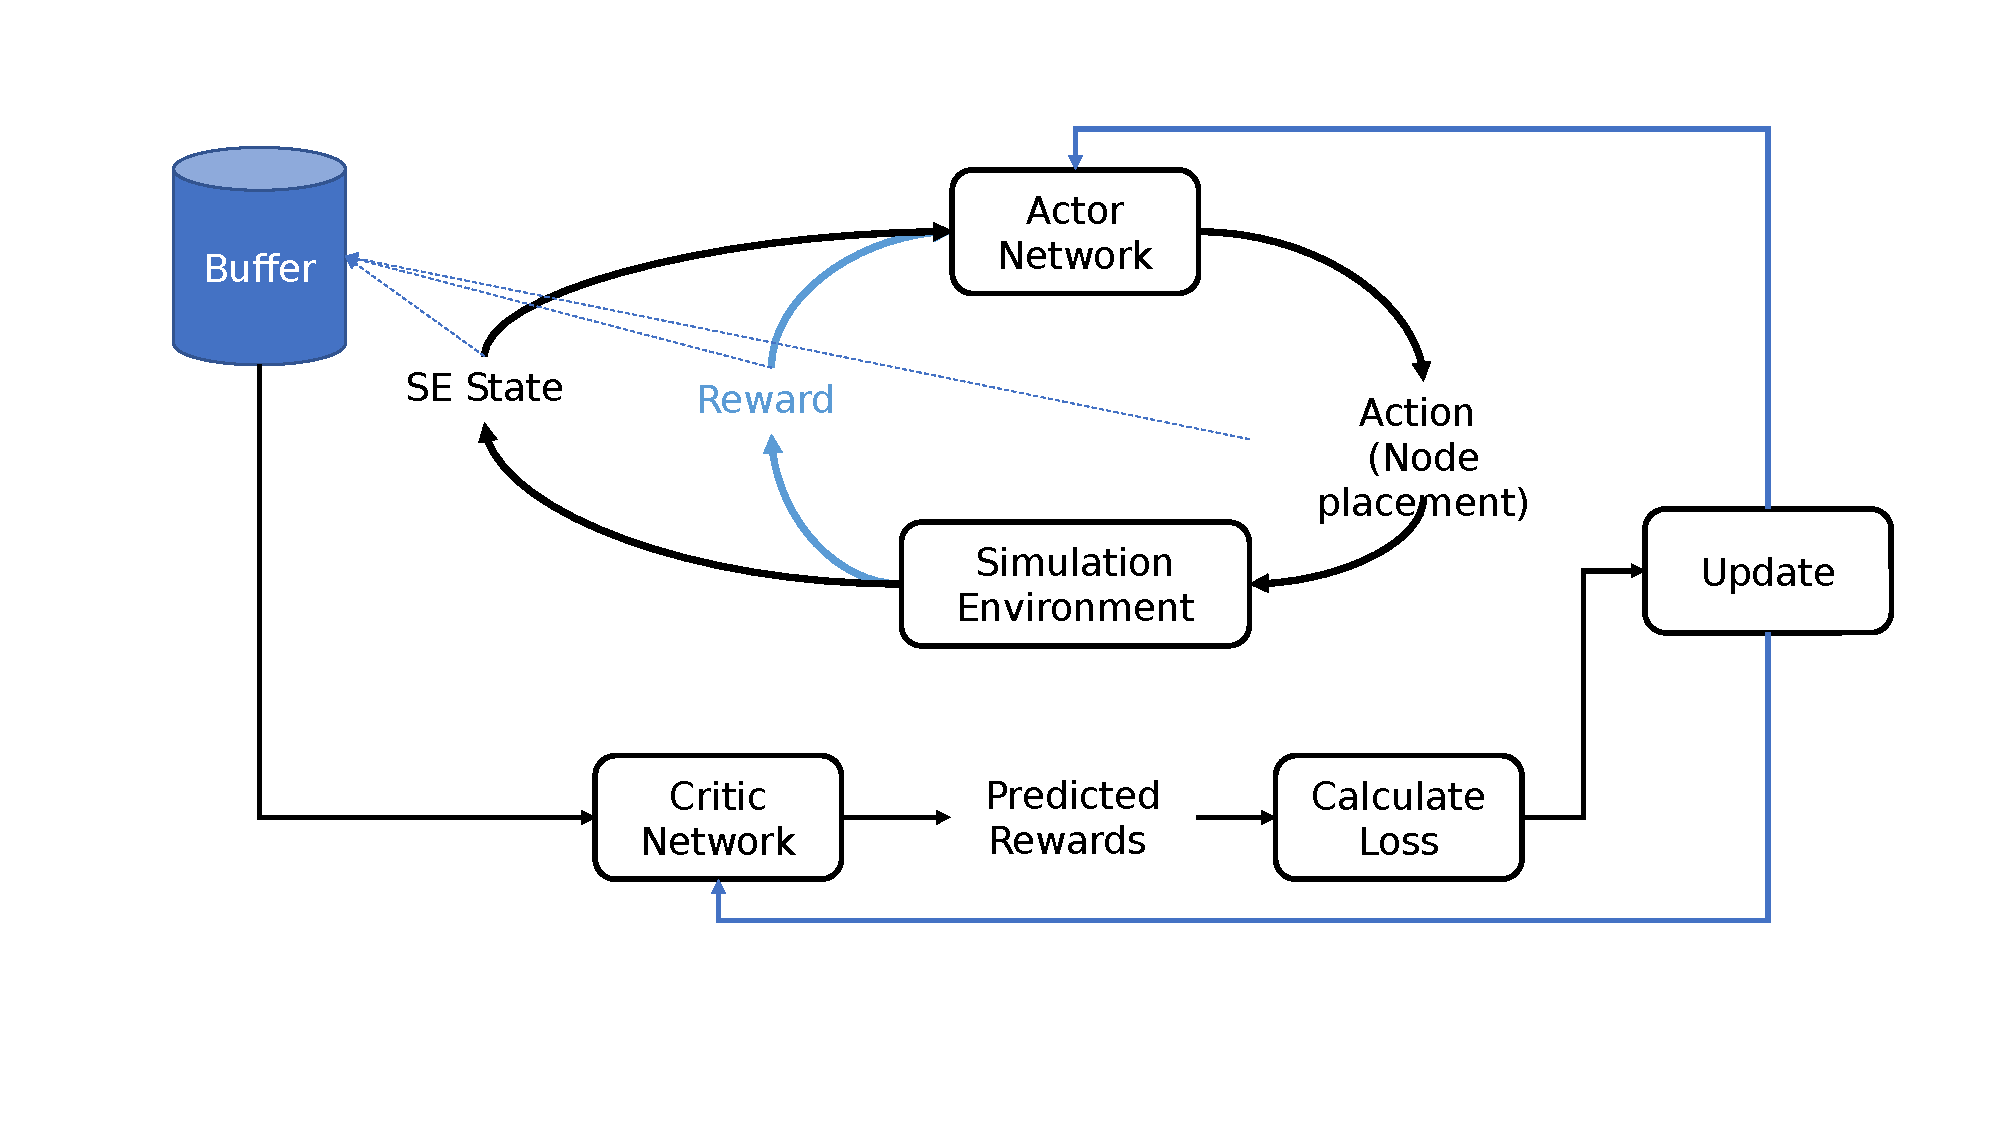
\includegraphics[width=\linewidth]{fig/ppo.pdf}
  \caption{Diagram of the RL framework showing the role of actor and critic networks during RL training. }
  \label{fig:ppo}
\end{figure}
\subsection{Model design}

The actor and critic models architecture is shown in figure \ref{fig:model}. 
The input is separated in two categories: static and dynamic data. 
Static data is information that doesn't change as nodes are being placed, such as: computation graph and tile memory constraint.
Device state, node to be placed and placed node latencies are dynamic data that changes during placement.

Tile memory variables need to be placed in a tile so that operation can use that variable. 
This memory constraint is captured as memory dependency array. 
Tile memory constraints are incorporated into nodes in the computation graph. 
The computation graph has each node representing an instruction. 
The node features are tile memory dependencies. 
A Graph Neural Network (GNN) is used to process node dependencies and create an embedding for each node. 
An attention module is applied to the embedding matrix to select which dependency nodes are relevant to the current node to be placed. The dynamic data is fed into a MLP model to 
create another embedding to represent current state. 
The two embeddings are combined and fed into another MLP model to 
create actions. 
Invalid actions are masked before being sent to the reward function. Masking was shown to be effective in RL setting \cite{Shengyi_mask}.

\begin{figure}[h]
  \centering
  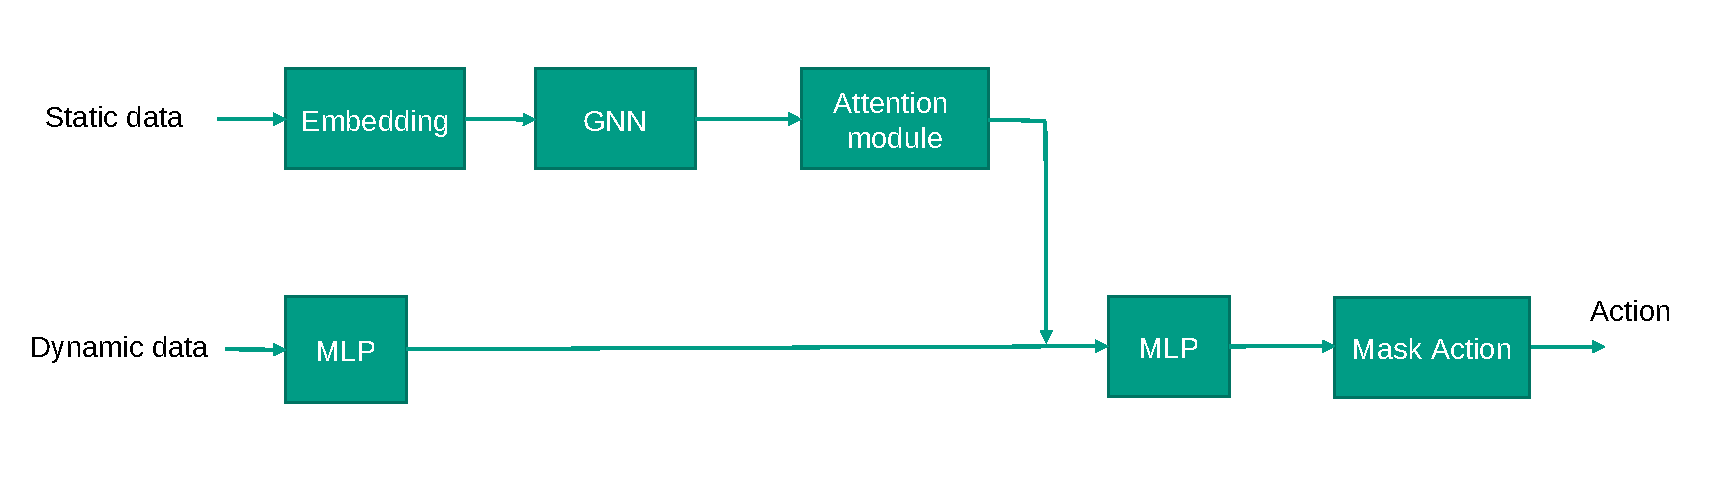
\includegraphics[width=\linewidth]{fig/model.pdf}
  \caption{Actor and critic model architecture. GNN is used to process the computation graph (static data). 
  Attention module gives importance to relevant nodes. The embedding created from dynamic data is combined with static data embedding. 
  A final MLP model is used to generate actions. Actions are masked to ensure only valid actions are produced. }
  \label{fig:model}
\end{figure}

